%
% lagrangezyl.tex -- 
%
% (c) 2024 Prof Dr Andreas Müller
%
\begin{figure}
\centering
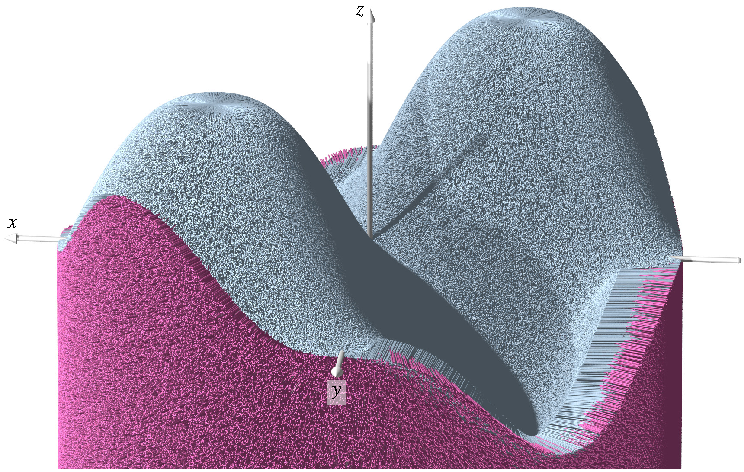
\includegraphics{chapters/010-fuvar/images/lagrangezyl.pdf}
\caption{Extremalproblem mit Nebenbedingung wie in
Abbildung~\ref{buch:fuvar:nebenbedingungen:fig:lagrangekurve}.
Zusätzlich zu den Flächen sind die Richtungen des Gradienten  von
$f(x,y)$ als blaue ``Haare'' und die Richtungen des Gradienten der
Nebenbedingung $g(x,y)$ als rote ``Haare'' dargestellt.
Die Extrema befinden sich dort, wo die Haare parallel sind.
Auf beiden Seiten des Maximums divergieren die ``Haare'', so dass
ein Spalt entsteht.
Auf beiden Seiten des Minimums überschneiden sich die Haare dagegen.
\label{buch:fuvar:nebenbedingungen:fig:lagrangezyl}}
\end{figure}
